\section{LHC Layout and Design} \label{sec:lhc:layout}

While often depicted as a perfect circle the LHC is in reality an octagon with
rounded edges, called arcs, as can be seen in \cref{fig:lhc_schematic}.
Here you can see the counter circulating beams of protons depicted in red and
blue.  These beams are focused and collided at the 4 dedicated interaction
points at rates of up to 40 MHz.  Two of these points are occupied by the
ATLAS and CMS experiments, both of which are high luminosity, multi-purpose
experiments.

\begin{figure}[!htbp] 
  \begin{center}
    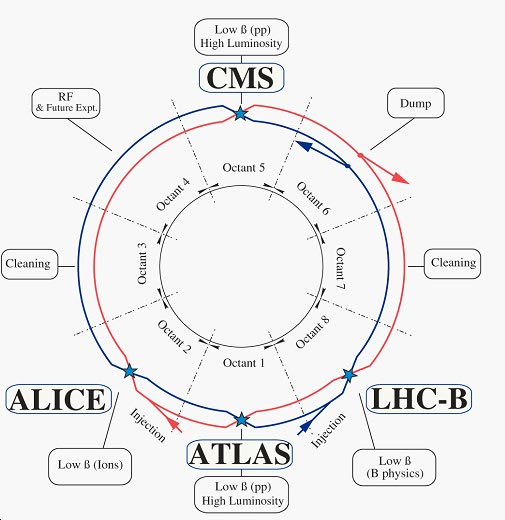
\includegraphics[width=0.9\linewidth]{figures/lhc/lhc_schematic.jpg}
    \caption{Labeled diagram of all the experiments at the LHC indicating the
counter circulating beams and points of interest along the circumference of the
accelerator.} 
    \label{fig:lhc_schematic} 
  \end{center} 
\end{figure}

The exact design of the LHC tunnel is due to the experimental constraints of the
original machine for which it was built, the Large Electron Positron (LEP)
Collider.  For the $\sim 2,000$ times lighter electron the maximum energy was
limited by the synchrotron radiation, proportional to $\frac{1}{m^4}$, requiring
long straight sections of accelerating RF cavities to recuperate the lost
energy.  Given that this effect is $\mathcal{O}(10^{13})$ times smaller for the
proton the LHC is instead limited by our ability to design and construct magnets
strong enough to bend the beam given the already determined curvature of the 8
arcs.

\begin{figure}[!htbp] 
  \begin{center}
    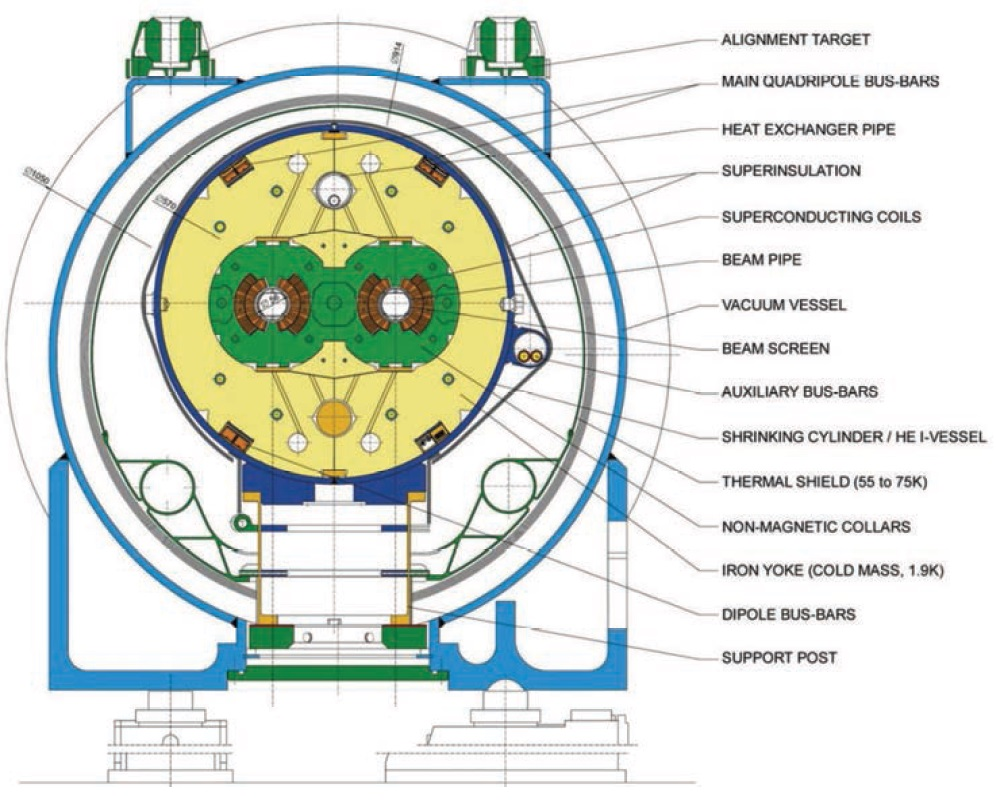
\includegraphics[width=0.9\linewidth]{figures/lhc/dipole.jpg}
    \caption{ Depiction of a LHC dipole magnet 2-in-1 design labeling the major
components} 
    \label{fig:dipole} 
  \end{center} 
\end{figure}

The oppositely circulating beams must each  have their own ring and magnetic field
which lead to the creation of a twin-bore (i.e. "two-in-one") magnet design, a
cross section of which can be seen in \cref{fig:dipole}. These magnets are constructed
using NbTi superconductors which are cooled to 2K using superfluid helium.
These magnets are designed to provide the needed 8.33 T magnetic field required
to bend the proton trajectories at the designed beam energy of 7 TeV.  In total 1231 of these 15
m bending dipole magnets are used, in association with 392 5-7m
quadrupole magnets which are responsible for keeping the proton bunches in a
tight beam by squeezing them both horizontally or vertically.
